% !Mode:: "TeX::UTF-8"
\documentclass[myposter,portrait]{sciposter}

%% uzitocne package
\usepackage{multicol}
\usepackage{color}
\usepackage{graphicx}

%% znaky s diakritikou
\usepackage[utf8]{inputenc}
\usepackage[T1]{fontenc}
\usepackage[slovak]{babel} % slovenske delenie slov

%% definicia farieb
\definecolor{mainCol}{rgb}{.97,.99,0.93} % farba pozadia posteru
\definecolor{BoxCol}{rgb}{.7,1,.7} % farba boxu okolo nadpisov
\definecolor{sectionCol}{rgb}{.5,.7,.5} % farba nadpisu
\definecolor{textCol}{rgb}{0,0.1,0} % farba hlavneho textu

\def\mysection#1{
{\color{sectionCol}\section*{\sc\bfseries #1}}}

\begin{document}
\setlength{\logowidth}{20cm}
\setlength{\titlewidth}{\textwidth}
\addtolength{\titlewidth}{-\logowidth}
\rightlogo[0.9]{images/fmfilogo-farebne}
\useleftlogofalse

\color{textCol}
\title{Zarovnávanie sekvencií s~použitím metód klasifikácie}

\author{Michal Hozza\\
  Školiteľ: Tomáš Vinař$^1$\\
  Konzultant: Michal N\'an\'asi$^2$}

\institute{
$^1$ Katedra aplikovanej informatiky,
FMFI UK, Mlynská Dolina, 842~48~Bratislava\\
$^2$ Katedra informatiky,
FMFI UK, Mlynská Dolina, 842~48~Bratislava}
\maketitle

\begin{multicols*}{3}

\mysection{Úvod}

Zarovnávanie dvoch DNA sekvencií je jedným zo základných
bioinformatických problémov. Správne zarovnanie identifikuje časti
sekvencie, ktoré vznikli z~toho istého predka (zarovnané bázy), ako aj
inzercie a delécie v~priebehu evolúcie (medzery v~zarovnaní). Obvykle
takéto zarovnanie hľadáme pomocou jednoduchých párových skrytých
Markovovských modelov (pHMM) \cite{durbin}. V~tejto práci sa zaoberáme
možnosťami použitia prídavnej informácie o~funkcii vstupných sekvencií
(tzv. anotácie) na zlepšenie kvality takýchto zarovnaní.

\mysection{Klasifikácia na základe lokálnej informácie.}

Informácie sme zakomponovali pomocou klasifikátorov, ktoré rozhodujú či dané pozície majú byť zarovnané k~sebe alebo nie. Ako klasifikátor sme použili \emph{RandomForest} \cite{randomForestPaper}, pretože aktuálne patrí medzi najlepšie klasifikátory.

Vstupné dáta pre klasifikátor sú okná veľkosti $w$, v ktorom sa nachádza $w$ dvojíc báz v okolí daných pozícií a ich anotácie (napr. či ide o gén alebo nie). Výstup je hodnota z intervalu $\left<0,1\right>$, ktorá označuje istotu klasifikátora, že dané dve pozície majú byť zarovnané k sebe (v insert stave, že daná pozícia má byť zarovnaná k medzere).

Ukázalo sa, že klasifikátor sa dokáže naučiť, ktoré okná majú byť zarovnané k~sebe a ktoré nie (Obr. \ref{fig:clf-m-dist}).

\begin{figure}[htp]
    \centering
    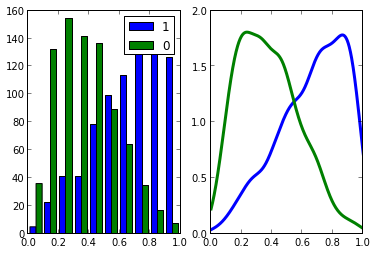
\includegraphics[width=\textwidth, clip=true]{images/clf_m_test}
    \caption{Distribúcia výstupu klasifikátora pre pozitívne a negatívne príklady. Pozitívne príklady sú tie, ktoré majú byť zarovnané k~sebe, negatívne príklady sú tie, ktoré k sebe zarovnané byť nemajú.}
    \label{fig:clf-m-dist}
\end{figure}

\mysection{Zakomponovanie výsledkov klasifikácie do pHMM.}

Vyvinuli sme 2 modely pre zarovnanie sekvencií s~anotáciami za pomoci klasifikátora, ktoré sú založené na párových skrytých Markovovských modeloch.

\paragraph{Model s~klasifikátorom ako emisiou:} (Obr. \ref{fig:model-clf})
V~tomto modeli sme nahradili emisné tabuľky stavov výstupom z~klasifikátora.
Model však nie je korektný pravdepodobnostný model, pretože pravdepodobnosti emisií nesčitujú do~1.

Emisné pravdepodobnosti sme prevzali priamo z klasifikátora, ktorý trénujeme zvlášť. Prechodové pravdepodobnosti sme natrénovali zo zarovnaní z trénovacej vzorky.

\begin{figure}[htp]
        \centering
        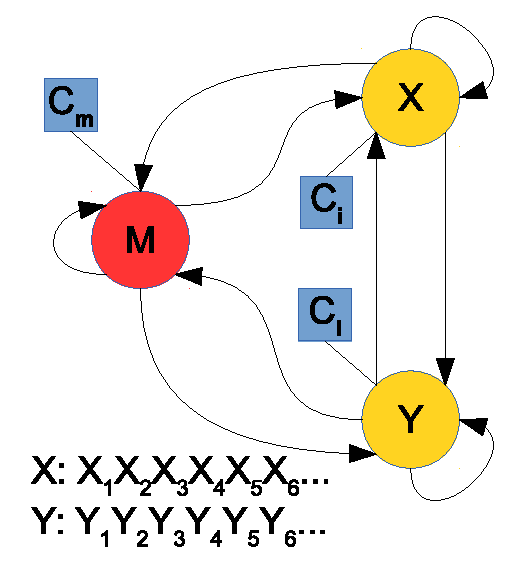
\includegraphics[width=.5\textwidth, clip=true]{images/model_clf}
        \caption{Model s~klasifikátorom ako emisiou}
        \label{fig:model-clf}
\end{figure}


\paragraph{Model s~klasifikátorovou páskou:} (Obr. \ref{fig:model-clf-tape})
Aby sme vyriešili problém s~korektnosťou predošlého modelu, navrhli sme alternatívu, ktorá navyše modeluje aj výstup z~klasifikátora.
Nemodelujeme teda len dvojicu sekvencií, ale aj sekvenciu výstupov klasifikátora.

V tomto modeli sme trénovali všetky parametre na trénovacej vzorke zarovnaní obohatenej o pásku s výstupmi z klasifikátora.

\begin{figure}[htp]
        \centering
        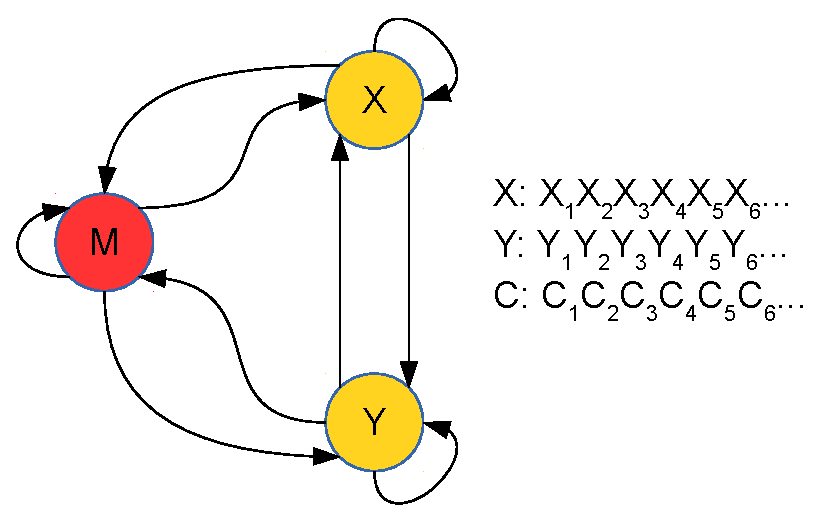
\includegraphics[width=.5\textwidth, clip=true]{images/model_clf_paska}
        \caption{Model s~klasifikátorovou páskou}
        \label{fig:model-clf-tape}
\end{figure}


%% zoznam literatury
\bibliographystyle{apalike}
\bibliography{references}

\end{multicols*}
\end{document}

